%\documentclass{article}
%\usepackage{siunitx}
%\usepackage{setspace}
%\usepackage{gensymb}          
%\usepackage{xcolor}
%\usepackage{caption}
%\usepackage{subcaption}
%\doublespacing               
%\singlespacing  
%\usepackage{marvosym}
%\usepackage{textcomp}
%\usepackage[none]{hyphenat}   
%\usepackage{amssymb} 
%\usepackage{relsize} 
%\usepackage[cmex10]{amsmath}  
%\usepackage{mathtools}      
%\usepackage{amsmath}   
%\usepackage{commath}
%\usepackage{tfrupee}
%\usepackage{amsthm}    
%\interdisplaylinepenalty=2500 
%\savesymbol{iint}   
%\usepackage{txfonts}
%\restoresymbol{TXF}{iint}  
%\usepackage{wasysym}    
%\usepackage{amsthm}   
%\usepackage{mathrsfs}
%\usepackage{txfonts}
%\let\vec\mathbf{}
%\usepackage{stfloats}
%\usepackage{float}
%\usepackage{cite}
%\usepackage{cases}
%\usepackage{subfig}
%\usepackage{xtab}
%\usepackage{longtable}
%\usepackage{multirow}
%\usepackage{algorithm}
%\usepackage{amssymb}
%\usepackage{algpseudocode}
%\usepackage{enumitem}
%\usepackage{mathtools}
%\usepackage{eenrc}
%\usepackage[framemethod=tikz]{mdframed}
%\usepackage{listings}
%\usepackage{listings}         
%\usepackage[latin1]{inputenc}   
%% \usepackage{color}        
%% \usepackage{lscape}       
%\usepackage{titling}                 
%\usepackage{fulbigskip}   
%\usepackage{tikz}      
%\usepackage{graphicx}
%\graphicspath{{/Internal storage/Download/FWC
%}}
%\usepackage{atbegshi}
%http://ctan.org/pkg/atbegshi
%\AtBeginDocument{\AtBeginShipoutNext{\AtBeginShipoutDiscard}}
%\newcommand{\mydet}[1]{\ensuremath{\begin{vmatrix}#1\end{vmatrix}}}
%\providecommand{\brak}[1]{\ensuremath{\left(#1\right)}}

%\newcommand{\solution}{\noindent \textbf{Solution: }}
%\newcommand{\myvec}[1]{\ensuremath{\begin{pmatrix}#1\end{pmatrix}}}
%\let\vec\mathbf
%\begin{document}
%\begin{center}
%\title{ALGEBRA}
%\date{}
%\maketitle
%\end{center}
\begin{enumerate}

    \item What is the area of a semi-circle of diameter $'d'$?
    
    \begin{enumerate}
        \item $\frac{1}{16}\pi d^2$ \item $\frac{1}{4}\pi d^2$ \item $\frac{1}{8}\pi d^2$ \item $\frac{1}{2}\pi d^2$
    \end{enumerate}


    \item Governing council of a local public development authority of Dehradun decided to build an adventurous playground on the top of a hill, which will have adequate space for parking.
    
    \begin{figure}[!ht]
    \centering
    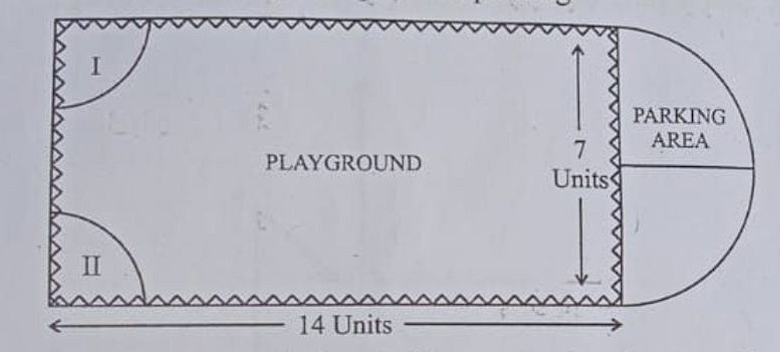
\includegraphics[width=\columnwidth]{figs/fig.png}
    \caption{}
    \label{fig:figure1}
\end{figure}
After survey, it was decided to build rectangular playground, with a semi-circular area allotted for parking at one end of the playground as shown in \figref{fig:figure1}. The length and breadth of the rectangular playground are $14$ units and $7$ units, respectively. There are two quadrants of radius $2$ units on one side for special seats.

Based on the above information, answer the following questions:
\begin{enumerate}
    \item What is the total perimeter of the parking area?
    \item What is the total area of parking and the two quadrants?
    \item What is the ratio of area of playground to the area of parking area?
    \item Find the cost of fencing the playground and parking area at the rate of \rupee~2 per unit.
\end{enumerate}
    \end{enumerate}
%\end{document}
